\documentclass[10pt,a4paper]{article}

\usepackage[latin1]{inputenc}
\usepackage{graphicx}

\frenchspacing
\sloppy
\pagestyle{plain}

\title{SICS AssertionServer}
\author{Ludwig Seitz \\SICS}

\begin{document}


\maketitle


\section*{\center \small Abstract}

{\small 
The SICS AssertionServer is a lightweight SAML-based identity management tool.
It's main purpose is to store and manage attribute information and issue
SAML attribute assertions for the stored attribute information.

AssertionServer provides pluggable modules for authenticating and authorizing
management of the attribute data it maintains. Example implementations of
these modules are provided.

The SICS Assertion Server is not a stand-alone product, rather is should be 
exposed as a service through a user-friendly interface and tied into a security
architecture, that consumer the assertions it produces.
}

\section{Introduction}
There a numerous commercial (and probably several open-source) solutions for 
identity management. However most of these (in fact all known to the author)
are very heavy-weight with lots of overhead, making them difficult to use
without extensive training.

Therefore we have decided to provide a lightweight identity management
service targeted at managing attributes and issuing SAML \cite{SAML2}
assertions for these attributes.

The architecture of the AssertionServer is shown in figure \ref{arch}

\begin{figure}[ht!]
  \centering
  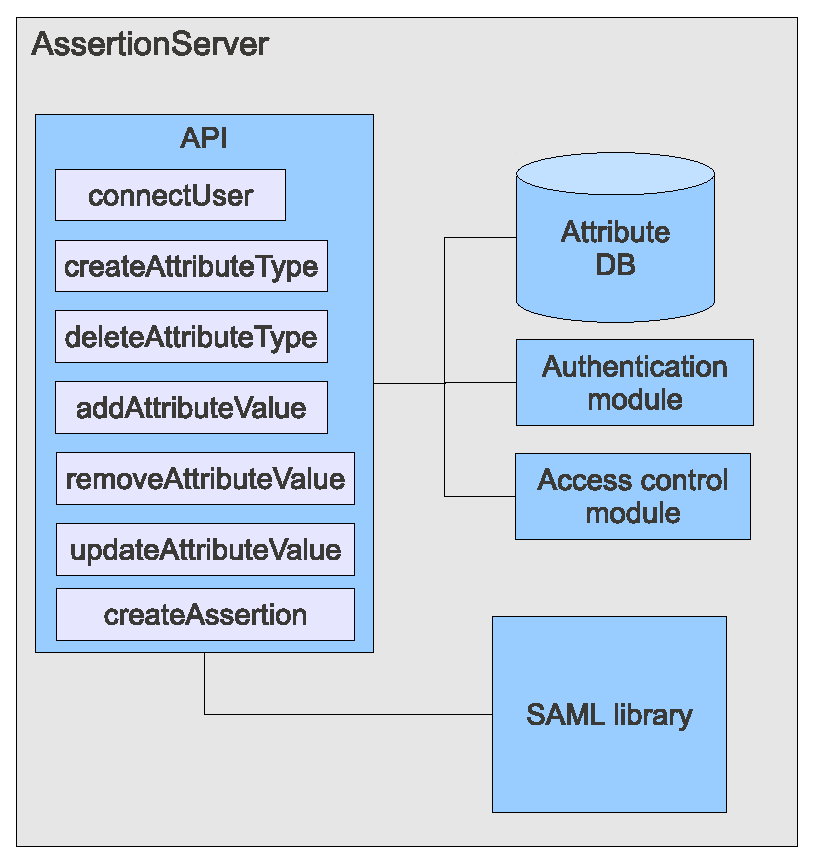
\includegraphics[scale=0.7]{ASarchitecture.eps}
  \caption{AssertionServer architecture}\label{arch}
\end{figure}

The elements of the architecture are as follows:

\begin{itemize}
  \item An API providing the main functions of the AssertionServer.
    This API is supposed to be exposed as a service (e.g. as a webservice).
  
  \item An attribute database. This database is managed via a pluggable 
    database connector.

    AssertionServer currently provides an example MySQL connector.
  
  \item An authentication module. This is used to authenticate users that want
    to access the API. The module plugs into an extension point, so that new
    types of authentication can easily be plugged in. We provide an example 
    module with password based authentication.
  
  \item An access control module. This is used to check the authorization of
    user that want to access the API. The module plugs into an extension point,
    so that new types of access control can easily be plugged in. We provide
    a simplistic example module where the owner of an attribute can perform
    any action, and other users can perfrom the \emph{createAssertion} function
    on arbitrary attributes.
   
  \item The \emph{SICS lighweight SAML library} (SlSl) is used to support the
    creation of attribute assertions.
\end{itemize}


\section{Concepts}
The following concepts are important in order to understand the purpose of 
AssertionServer. As an identity management tool, assertion server manages 
\emph{Attributes} assigned to \emph{Subjects}. Examples of subject attributes 
could be their age, security clearance, or role.

An \emph{Attribute} is defined as a tuple of \emph{Source of authority},
\emph{attribute identifier}, \emph{datatype} and \emph{attribute value}.

The \emph{Source of authority} (SOA) of an attribute defines the subject
that is in control of this attribute (i.e. that can decide over the
assignment of attribute values to other subjects).

The \emph{attribute identifier} is the name of the attribute e.g. \emph{Age},
or \emph{Security-Clearance} or \emph{Role}.

Each attribute has a specific \emph{Datatype} that constraints the set of
possible values for this attribute. For example age has the datatype integer 
(while it could even be further constrained to positive integers).

An \emph{Attribute Value} is the value of an attribute assigned to a subject.
E.g. For \emph{subject = Ludwig} and the \emph{attribute identifier = role}
an attribute value could be \emph{senior researcher}.

An \emph{Attribute Definition} defines the SOA, attribute identifier, datatype,
and optionally a set of allowed values for the attribute. Note that the 
attribute definition does not contain any assignments of attribute values to
subjects. 

The assertion server requires you to create an attribute definition, before you
start to assign attribute values for this attribute.

SAML assertions are signed XML documents that bind an attribute to a subject.
The issuer of the SAML assertion, asserts that the subject has the named
attribute, e.g. \emph{SICS (issuer) says that Ludwig (subject) has the role 
(attribute-identifier) "senior researcher" (attribute value)}.

The SAML standard is defined by the OASIS standardization organization, and
is described in numerous documents available on the web.

\section{Configuration}\label{configure}
In order to operate the SICS AssertionServer you need to perform a small number
of configuration steps:

\begin{enumerate}
  \item Install the MySQL database server and create a user for the 
    AssertionServer. By default this user is called \emph{saml-aa} in
    the AssertionServer code, but this value is configurable.
  \item Get an instance of the \texttt{DBConnector} class and run the 
    \texttt{init(String)} method in order to create the necessary tables. 
    See \ref{DBConnector} for details.
  \item Select an authentication module and configure it. See \ref{AAA} for
    details.
  \item Select an access control module and configure it. See \ref{AAA} for 
    details.
  \item Create a pair of assymetric keys for the AssertionServer. These will
    be used for signing SAML assertions.
\end{enumerate}

After this you can create an instance of the \texttt{AssertionServer} class and
use the functions provided by the API.

\subsection{Database Connectors}\label{DBConnector}
The AssertionServer needs a database connector in order to store information
on a database. The connector needs to implement the \texttt{DBConnector}
interface.

We provide the class \texttt{SQLConnector} that uses the Interfaces from the 
\texttt{java.sql} package. 

In order to make this work with a concrete database you need to put a JDBC-jar
in the build path. We have tested SQLConnector with the \emph{MySQL} database 
and the \texttt{mysql-connector-java.jar} JDBC library.

\subsection{AAA-modules}\label{AAA}
AssertionServer supports pluggable modules for Authentication and Access 
Control. Furthermore Accounting is supported by configurable logging 
with the Log4j library.

The Authentication module needs to implement the \texttt{AuthenticationModule}
interface, while the Access Control module needs to implement 
\texttt{AccessControlModule}. Both modules require that you run the 
\texttt{init(DBConnector)} method first, in order to create necessary database
tables for the authentication or access control data.

The Access Control module trusts the previous authentication of a user by the
Authentication module, and obtains the user-id of the currently connected user 
from the \texttt{AssertionServer} class. 


We provide simplistic example modules and encourage the development of more 
sophisticated ones. 

The \texttt{PasswordAuth} class implements password-based authentication. 
The authentication token passed to the \texttt{newUser()} and \texttt{doAuth()}
methods of this class must be the raw password as
a \texttt{String}.

The \texttt{BasicAccessControl} class implements a policy, where the 
source of authority (SOA) of an attribute can do any operation on this
attribute, while other users can only retrieve SAML assertions.

\subsection{Certificates}
The AssertionServer requires a X.509 certificate and the associated secret key
in order to sign SAML assertions it issues. The certificate and the 
corresponding private key is expected to be encoded in a file in 
\emph{PKCS\#12} format (i.e. a \emph{.p12} file).

Furthermore you need to provide the root certificate(s) that was used to sign
the CA certificate as a Base64 encoded DER certificate (i.e. a \emph{.pem} 
file).

This information is used as parameters in the constructor of the 
\texttt{AssertionServer} class.

\section{Functions}
The AssertionServer API (from the \texttt{AssertionServer} class) supports the
following functions:

\begin{itemize}
  \item Connecting a User;
  \item Disconnecting a User;
  \item Creating an Attribute Definition;
  \item Deleting an Attribute Definition;
  \item Adding an Attribute Value;
  \item Removing an Attribute Value;
  \item Updating an Attribute Value;
  \item Getting a SAML Assertion.
\end{itemize}

They are described briefly in the following subsections.


\subsection{Connecting a User }
In order to perform any of the other functions of the AssertionServer
a user needs to establish a connection (and in the process of doing so
to authenticate). The method \texttt{connectUser(SAMLID, Object)}
allows a user to connect to the AssertionServer. The SAMLID is expected to
be the user identifier of the connecting user, while the Object can either
contain an authentication token, or information necessary to perform an
authentication protocol. 

The exact contents of the Object parameter are up to the Authentication module
(see \ref{AAA}).

After a user is connected, his identity is used to authorize any requests
until the user is disonnected.

Note that the AssertionServer does not support multiple administrative users
connected at the same time.

\subsection{Disconnecting a User}
The \texttt{disconnectUser()} method disconnects the current user.

\subsection{Creating an Attribute Definition}
The \texttt{createAttribute(AttributeDefinition)} method creates a new 
attribute definition. The \texttt{AttributeDefinition} parameter contains all
relevant information for this.


\subsection{Deleting an Attribute Definition}
The \texttt{deleteAttribute(AttributeDefinition)} method deletes an existing
attribute definition and all associated attributes. If the attribute definition
given as parameter does not exist, the AssertionServer returns an error 
message.

\subsection{Adding an Attribute Value}
The \texttt{addAttributeValue(SAMLID, SAMLID, SAMLAttribute)} method adds
a new attribute to a subject. The first SAMLID represents the subject,
the second the SOA of the attribute and finally the attribute is provided in
the SAMLAttribute parameter.

\subsection{Removing an Attribute Value}
The \texttt{removeAttributeValue(SAMLID, SAMLID, SAMLAttribute)} method 
removes an existing attribute from a subject. The first SAMLID represents
the subject, the second the SOA fo the attribute. Note that the SAMLAttribute
must specify the whole attribute (including the attribute value) in order
for this method to succeed.

\subsection{Updating an Attribute Value}
The \texttt{updateAttributeValue(SAMLID, SAMLID, SAMLAttribute, String)} method
updates an attribute. The first SAMLID represents the subject, the second the 
SOA fo the attribute. The SAMLAttribute parameter must contain the old
attribute, while the String parameter must contain the String representation
of the new attribute value.

\subsection{Getting a SAML Assertion}
The \texttt{getAssertions(AssertionRequest)} method generates SAML assertions
for existing attributes. Note that the \texttt{AssertionRequest} parameter
allows to set the attribute value to \texttt{null} in order to retrieve all 
attribute values for a specific attribute.

\section{Database structure}
Normally you shouldn't need to interact with the database directly, since the
DatabaseConnector should function as communication bridge. However for 
debugging and for a better understanding of the AssertionServer it can be 
useful to be aware of the structure of the database tables it uses.

AssertionServer uses two tables for attribute management. Additional tables may
be used by the authentication and authorization modules.

The \emph{attribute definition} table (default name: 
\emph{AttributeDefinitions}) stores the definitions of attributes.
It's fields are: \emph{attribute identifier}, \emph{source of authority}, 
\emph{datatype} and the set of allowed values for an attribute. Note that no 
actual attribute values are stored here.

The \emph{attribute value} table (default name: \emph{AttributeValue}) stores
the associations of attributes to subjects. It's fields are \emph{subject} 
(the identifier of the subject to which the attribute is associated), 
\emph{source of authority}, \emph{attribute identifier}, \emph{datatype},
and \emph{attribute value}.

The reason why we store all of \emph{source of authority}, \emph{attribute 
identifier} and \emph{datatype} is that an attibute is only uniquely defined 
by the combination of these values. Thus it is concievable that two SOA's would
have attributes with the same attribute identifier (and datatype). These
attributes would still be considered to be different.

Note that a subject could have several attriubute values for the same 
attribute, which would be represented by having several table entries, with 
identical \emph{subject}, \emph{source of authority}, \emph{attribute 
identifier} and \emph{datatype} fields, one for each attribute value.


\section{Code example}

\begin{verbatim}
//Use default values for connecting to the database
SQLConnector db =  new SQLConnector(null, null, null);

AccessControlModule pdp = new BasicAccessControl();

//Use the default hash algorithm on the passwords
PasswordAuth auth = new PasswordAuth(null);
	
List<X509Certificate> certs = new ArrayList<X509Certificate>();
File rootCertFile = new File("resources/testData/Certificates/cacert.pem");

CertificateFactory certFact = CertificateFactory.getInstance("X.509");
               
BufferedInputStream bis = new BufferedInputStream(
   new FileInputStream(rootCertFile));
        
X509Certificate rootCert 
   = (X509Certificate) certFact.generateCertificate(bis);
certs.add(rootCert);
        
AssertionServer sas = new AssertionServer(db, pdp, auth,
   "resources/testData/Certificates/aserver.p12",
   "password", certs, 1);
		
HashSet<String> allowedValues = new HashSet<String>();
allowedValues.add("member");
allowedValues.add("administrator");
		
SAMLNameID subject = new SAMLNameID("ludwig@sics.se");
String soaStr = "testSOA";
SAMLNameID soa = new SAMLNameID(soaStr);
String id = "testID";
String dataType = SAMLAttribute.xmlStringId;

//Add required XML-attributes for the SAML-XACML profile
HashMap<String, String> otherXMLAttrs = new HashMap<String, String>();
otherXMLAttrs.put("xmlns:" + SAMLAttribute.xacmlprofNSPrefix, 
   SAMLAttribute.xacmlprofNS);
otherXMLAttrs.put(SAMLAttribute.xacmlprofNSPrefix + ":" +
   "DataType", dataType);

ArrayList<SAMLAttributeValue> values
   = new ArrayList<SAMLAttributeValue>();
values.add(new SAMLAttributeValue(null, "member"));
SAMLAttribute valueMember = new SAMLAttribute(
   id, SAMLAttribute.xacmlNameFormat, null, 
   otherXMLAttrs, values);

values.clear();
values.add(new SAMLAttributeValue(null, "administrator"));
SAMLAttribute valueAdmin = new SAMLAttribute(
   id, SAMLAttribute.xacmlNameFormat, null, 
   otherXMLAttrs, values);

AttributeDefinition ad = new AttributeDefinition(soa, id, 
   dataType, allowedValues);
		
//Create the database
db.init("password");
auth.init(db);

//Create a new user
auth.newUser(ad.getSOA().getName(), "password", db);

//Authenticate the user
RequestResult result = sas.connectUser(ad.getSOA(), "password");
if (!result.success()) {
   System.out.println(result.getFailureReasons());
}
		
//Create an attribute
result = sas.createAttribute(ad);
		
if (!result.success()) {
   System.out.println("..." + result.getFailureReasons());
}
		
//Adding an attribute value
result = sas.addAttributeValue(subject, soa, valueMember);
if (!result.success()) {
   System.out.println("..." + result.getFailureReasons());
}
		
//Update an attribute value
result = sas.updateAttributeValue(subject, soa, valueMember,
   "administrator");
if (!result.success()) {
   System.out.println("..." + result.getFailureReasons());
}

//Get assertion
AssertionRequest request = new AssertionRequest(subject, soa, valueAdmin);
result = sas.getAssertions(request);
SignedSAMLAssertion assertion = result.getResults().get(0);
String assertionXML = assertion.toString(new Indenter());
System.out.println(assertionXML);
		
//Parse an assertion
XMLInputParser parser = new XMLInputParser(null, null);
Document doc = parser.parseDocument(assertionXML);
SignedSAMLAssertion parsedAssertion 
   = SignedSAMLAssertion.getInstance(doc.getDocumentElement());
		
//Test validity of conditions
if (!parsedAssertion.getConditions().checkValidityIntervall()) {
   // Failed
} else {
  // Success
}

//Delete an attribute value
result = sas.removeAttributeValue(subject, soa, valueAdmin);
if (!result.success()) {
   System.out.println(result.getFailureReasons());
}		

//Delete an attribute
result = sas.deleteAttribute(ad);
		
if (!result.success()) {
   System.out.println("..." + result.getFailureReasons());
}

//Delete a user
auth.deleteUser(ad.getSOA().getName(), db);
\end{verbatim}
\bibliography{references}
\bibliographystyle{ludwig}

\end{document}
